\documentclass[tikz,border=12pt]{standalone}
\usepackage[T1]{fontenc}
\usepackage{lmodern}
\usetikzlibrary{positioning,arrows.meta,shapes.geometric}

\begin{document}
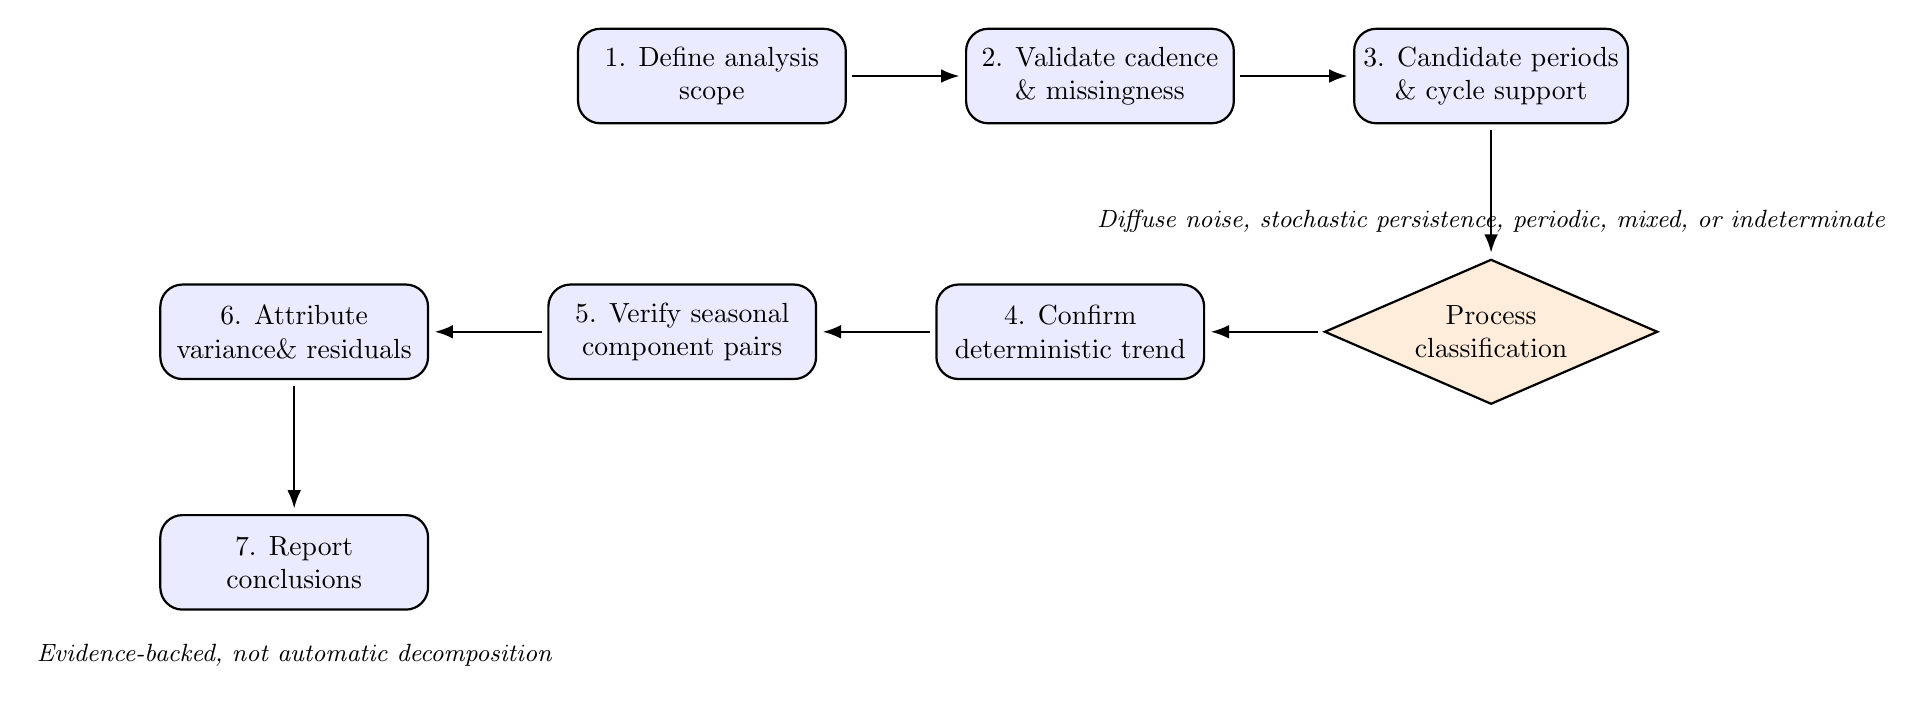
\begin{tikzpicture}[
  stage/.style={draw, rounded corners=8pt, align=center, minimum width=3.4cm, minimum height=1.2cm, fill=blue!8, line width=0.8pt},
  gate/.style={draw, diamond, align=center, aspect=2.3, fill=orange!14, line width=0.8pt},
  note/.style={font=\small\itshape, align=center},
  arrow/.style={-Latex, thick, shorten >=2pt, shorten <=2pt}
]

\node[stage] (scope) {1. Define analysis\\scope};
\node[stage, right=1.5cm of scope] (validate) {2. Validate cadence\\\& missingness};
\node[stage, right=1.5cm of validate] (periods) {3. Candidate periods\\\& cycle support};
\node[gate, below=1.7cm of periods] (classify) {Process\\classification};
\node[stage, left=1.5cm of classify] (trend) {4. Confirm\\deterministic trend};
\node[stage, left=1.5cm of trend] (season) {5. Verify seasonal\\component pairs};
\node[stage, left=1.5cm of season] (attrib) {6. Attribute\\variance\& residuals};
\node[stage, below=1.7cm of attrib] (report) {7. Report\\conclusions};

\draw[arrow] (scope) -- (validate);
\draw[arrow] (validate) -- (periods);
\draw[arrow] (periods) -- (classify);
\draw[arrow] (classify) -- (trend);
\draw[arrow] (trend) -- (season);
\draw[arrow] (season) -- (attrib);
\draw[arrow] (attrib) -- (report);

\node[note, above=0.2cm of classify] {Diffuse noise, stochastic persistence, periodic, mixed, or indeterminate};
\node[note, below=0.3cm of report] {Evidence-backed, not automatic decomposition};

\end{tikzpicture}
\end{document}
